\chapter{Synchronous Message Exchange}

In the previous chapter we went through the theory behind logic design, all the way from the introduction of Boolean algebra to gate-level implementation of logic units. In this chapter we will use those ideas to implement logic units in synchronous message exchange (SME). This will serve as a means to introduce SME to the reader and further cement former logic design ideas.

Starting out we will go through a short introduction behind the inspiration for SME, Communicating Sequential Processes. Hereafter we will go through the theory and syntax of SME with an emphasis on real examples, as I believe this is the most efficient manner of introducing SME to the reader.  

\section{Communicating Sequential Processes}
    
    When working with multiprocessor workloads, you will quickly realize the inconvenience of memory sharing. The non-determinism of having multiple processes reading and writing the same memory often results in unexpected behavior.
    
    A classic example of non-determinism would be the act of printing out the numbers one through ten, to your console using more than one thread. If the aforementioned code is executed multiple times, you will notice that the order of numbers would vary between the runs. This is due to the scheduler of the operating system, which we do not have control over. That can create race conditions (meaning the behavior in your code is dependent on the timing of different threads), which can cause unpredictable behavior and therefore bugs, which is undesirable.
    
    Various attempts has been made to solve this problem, such as the introduction of mutexes or locks. Though it does not solve our problem completely as these "solutions" introduces deadlocks, which is a state, where multiple processes are waiting for each other and the program stalls indefinitely. These deadlocks might not happen every run and thus introduces another layer of difficulty, as error reproducibility is essential for code debugging and therefore makes it hard to make reliable software.
    
    Communicating Sequential Processes (CSP) is an algebra first proposed by \citet{HoareC1978Csp} to solve exactly these issues.
    CSP is build on two very basic primitives, first is the process (which should not be confused with operating system processes). A process could be an ordered sequence of operations. These processes do not share any memory, therefore one process cannot access a specific value in another process (which solves the problems we had with shared memory).
    
    The other primitive is channels, which is the way the processes communicate with each other. You can pass whatever you want through these channels, but once you pass the value, the process lose access to it. There are a lot of ways the processes and channels can be arranged. The most simple can be found in figure \ref{fig:one_to_one}, which illustrates process 1 passing a value onto a channel, which process 2 takes as input. Some different configurations can be found in figures  \ref{fig:one_to_many}-\ref{fig:many_to_many}. 
    
    Using these primitives as the programming paradigm, multiprocess workloads can be designed without the shared memory problems mentioned earlier. The asynchronous nature of CSP will though be a problem for hardware models, as we will see shortly and is the fundamental inspiration behind Synchronous Message Exchange. 

    \begin{figure}[h!]
        \hspace*{-1.25cm}
        \begin{subfigure}[t]{0.5\textwidth}
            \centering
            \subimport{tikz_stuff/}{one_to_one}
            \caption{CSP one to one}
            \label{fig:one_to_one}
        \end{subfigure}%
        \hspace*{1cm}
        \begin{subfigure}[t]{0.5\textwidth}
            \centering
            \subimport{tikz_stuff/}{one_to_many}
            \caption{CSP one to many}
            \label{fig:one_to_many}
        \end{subfigure}
        \vspace*{2cm}
        
        \hspace*{-1cm}
        \begin{subfigure}[b]{0.5\textwidth}
            \centering
            \subimport{tikz_stuff/}{many_to_one}
            \caption{CSP many to one}
            \label{fig:many_to_one}
        \end{subfigure}%
        \hspace*{1cm}
        \begin{subfigure}[b]{0.5\textwidth}
            \centering
            \subimport{tikz_stuff/}{many_to_many}
            \caption{CSP many to many}
            \label{fig:many_to_many}
        \end{subfigure}%
    \end{figure}
    
\section{Synchronous Message Exchange}
    The idea of using CSP for hardware modeling was first introduced in \citet{BPUSimulator2013} and later further developed in \cite{PyCSPFPGA}, where two students successfully implemented a vector processor using PyCSP (a CSP library for python). They however found a number of shortcomings of using PyCSP for hardware modeling. The need for global synchronicity, when simulating hardware models using CSP, meant that additional channels were needed to simulate clock progress and emulation of latches among others. This caused an explosion of required channels and processes, which is an unnecessary increase in complexity.
    
    They did however find that building isolated processes and then connecting them via channels proved to be a powerful approach for building larger hardware models. As in the unit testing method one can develop and test individual processes to then connecting them together and form larger hardware models.
    
    With this in mind a more suitable message-passing framework for hardware modeling was developed, with the following requirements:
    
    \begin{itemize}
        \item Globally synchronous
        \item Broadcasting channels
        \item Shared nothing
        \item Implicit latches
    \end{itemize} 
    
    all these observations laid the foundation behind Synchronous Message Exchange (SME),  \citet{vinter2014synchronous}. 
    Since then the SME framework has been implemented in the .NET framework, \citet{skovhede2016building}, which is the version of SME that will be used throughout this thesis.
    
    We will not dwell further into the theory behind SME in this thesis. Instead we will be developing actual units in SME, that will be needed when we later implement the RISC-V architecture. The SME syntax will be introduced as we go through the examples and is intended to be a from-scratch introduction for the uninitiated reader. 
    
    \note{beskriv clocked proceser der trigger ikke clocked processer plus nævn skjult bus, skriv hvad latch er}
    \note{beskriv rendevouz og broadcast}

    \subsection{SME setup and structure}
        We will in this section go through the code structure I have decided to use for the development of all logic units. Much thought has been given to this and from previous experience doing code projects I would say it is good practice to think about the general structure of the project for ease of development and future extensions.
        
        A modular design is essential, as many logic units is going to be needed when implementing the RISC-V architecture. This also allows for easy debugging and testing, as individual units can be addressed before integrating them into a larger system. Each logic unit will also be separated into two files. One which contains all the buses and one which contains the function of the unit. The thought behind this is to help compartmentalize bus declarations from unit function and hopefully ease development.  
        
        In the following it is a prerequisite that .NET Core SDK\footnote{The SDK can be found here \url{https://dotnet.microsoft.com/download}} is installed on their respective systems to be able to run the code. All following code examples can be found by clicking \href{https://github.com/DanielRamyar/Master_Thesis/tree/master/SME_Implementations}{here} or if reading printed version the full link can be found in this footnote\footnote{\url{https://github.com/DanielRamyar/Master_Thesis/tree/master/SME_Implementations}}.
        
        In the following it should be noted that the equivalent to a channel in CSP, is a bus in SME. Buses however, are able to contain multiple signals/channels.  
        
        \subsubsection{Project structure example}
        We are going to build an AND gate for this example. This will be the only section were the complete code is shown, as this section is meant to serve as a "quick start guide" for readers beginning their journey into SME. Subsequent sections will only show relevant parts of the code. 
        
        For this quick example we are going to start a project in a folder called \texttt{.../ANDGate/}, which is where all shown files are going to be placed.
        To do this we are going to open up a terminal window and navigate to the desired folder destination (for example the Desktop) and invoke the command: 
        
        \begin{lstlisting}[language=bash]
$ dotnet new console -n ANDGate
        \end{lstlisting}
        where "\texttt{ANDGate}" can be changed to a name of choice.
        
        Next navigate into the folder
        \begin{lstlisting}[language=bash]
$ cd ANDGate 
        \end{lstlisting}
        and add the necessary SME libraries
        \begin{lstlisting}[language=bash]
$ dotnet add package SME --version=0.4.0-beta
$ dotnet add package SME.GraphViz --version=0.4.0-beta
$ dotnet add package SME.Tracer --version=0.4.0-beta
$ dotnet add package SME.VHDL --version=0.4.0-beta
        \end{lstlisting}
        
        There should now exist 3 items inside the \texttt{ANDGate} folder: \texttt{Program.cs}, \texttt{ANDGate.csproj} and a folder called \texttt{obj}. If all went well we should now be able to begin with our project.
        
        I always find drawing a quick flowchart before implementing code gives a nice overview the project. So in the spirit of this I've drawn out a quick sketch of the project in Figure \ref{fig:ANDGateSME}, which shows the two processes we are going to create, namely the SME simulator and the AND gate process.
        
        \begin{figure}[h!]
            \vspace*{-1.5cm}
            \centering
            \subimport{tikz_stuff/}{ANDGateSME}
            \caption{Flowchart of AND gate SME project. Here the rectangles represent individual processes, which lies in a file of its own. The solid arrow represents a bus and dashed arrow a bus going to a clocked process.}
            \label{fig:ANDGateSME}
        \end{figure}  
        
        
\newpage
        Opening up the \texttt{Program.cs} file, we are going to add a couple of lines, as shown in Listing \ref{projectfile}. The \texttt{Program.cs} contains the \texttt{Main()} method of the project and is the entry point of any C\scalerel*{\#}{X} program. To use the SME library we import it with the "\texttt{using SME}" command as shown in the second line. 
        
        Within the \texttt{Main()} method, the first function we meet is the using function, this is just to ensure the resources is properly cleaned up after the simulation.
        
        Hereafter we see the simulation object, which as the name implies, is responsible for the simulation of the logic unit. We then pass the simulated input to the \texttt{ANDgate} object, which will then perform the AND operation (it is not necessary to pass the simulation object itself to the \texttt{ANDGate}, but is shown here to not cause confusion about how the simulation passes input values to the AND process). We will see how these objects are defined shortly. 
        
        Lastly we can configure the simulation with the sim object, which uses fluent syntax. In this case we configured it to build a CSV file, which shows what each bus contained at every clock cycle. We build a graph, which outputs a \texttt{.dot} file that shows how all the processes are connected and we transpile the code to VHDL. It should be noted that \texttt{Run()} should always be the last method called.
        
        The file which contains the \texttt{Main()} will ways be named \texttt{program.cs} in this thesis, but the naming is irrelevant.
        
        
        \lstinputlisting[language={[Sharp]C}, caption={The \texttt{Program.cs} file, which contains the \texttt{Main()} method for the project.},captionpos=b, label = projectfile]{/Users/danielramyar/Desktop/Thesis/SME_Implementations/ANDGate/Project.cs}  

        We are going to need a way to test our AND gate, this is what the simulation file is for and is shown in Listing \ref{simulatorfile}. Remember to name your \texttt{namespace} the same as in the project file. The first two definitions inside the simulation process creates or loads the two buses for the test. Notice that the gate output is labeled as an input bus and vice versa for the gate input. This is due to the simulation is a process in and of itself and therefore needs to output the test values to a bus, which the \texttt{ANDGate} process takes in as input.
        
        Now everything within the \texttt{Run()} method is what is going to be simulated and each time we want a new clock cycle to occur, we use the line \texttt{await ClockAsync()}. In a simulation process any .NET library is allowed and is not going to get transpiled to a VHDL file. Therefore we can print the output of the AND gate to console to see whether or not it works correctly. We do this by transmitting data via the input bus, which contains two signals, \texttt{in1} and \texttt{in2}. We then set the two signals to false wait a clock cycle and print the output. Since this is a fairly small system we can test for all input combinations and look at the outputs to see if the gate is behaving correctly. 

\begin{lstlisting}[language={[Sharp]C}, caption={The simulator file, which specifies how the simulation is run. Most lines in the run method are concatenated brievity.},captionpos=b, label = simulatorfile]
using System;
using SME;

namespace ANDGate {
    public class ANDGateSimulator : SimulationProcess {
        [InputBus]
        public readonly GateOutput output = Scope.CreateOrLoadBus<GateOutput>();
        
        [OutputBus]
        public readonly GateInputs input = Scope.CreateOrLoadBus<GateInputs>();
        
        public async override System.Threading.Tasks.Task Run() {
            Console.WriteLine("Starting test!\n");
            await ClockAsync();
            
            input.in_1 = false;
            input.in_2 = false;
            
            await ClockAsync();
            Console.WriteLine($"Gate input: {input.in_1} (Input 1) - {input.in_2} (Input 2)\n");
            Console.WriteLine($"AND gate output: {output.out_AND}");
            ... (Abbreviated the code here for space concerns)
            Console.WriteLine("Done testing!");
        }
    }
}
\end{lstlisting}
\newpage
        Hereafter we are going to make our bus declarations in a new file called buses.cs. Looking at Listing \ref{busdeclarations}, we see that the bus declarations are made using the interface command, which inherits its fields and methods from the \texttt{IBus} interface. The name for the bus is free of choice and in this case are called \texttt{GateInputs} and \texttt{GateOuputs} respectively.
        
        A bus can contain multiple signals of various types. Since the AND gate evaluates binary values, the \texttt{bool} type has been chosen for the input and output signals. You may have noticed that all the signals have the \texttt{InitialValue} attribute. What this does is that once the bus is created it will contain an initial value. If this is not done you have to be careful not to read the bus before any value has been given to it, as this will crash the program.
        
        Hereafter we have the \texttt{TopLevelInputBus} and \texttt{TopLevelOuputBus} attributes, they tell SME which buses goes in and out of the hardware implementation. Remember that this attribute is only given to buses which interfacing with some outside process, in this case the simulation process. Internal buses should not be given this attribute. By a internal bus we mean a bus which is connecting processes inside the hardware implementation (see Figure \ref{fig:2BitDecoderSME} here the internal buses goes from the NOT gates to the AND gates).

        \lstinputlisting[language={[Sharp]C}, caption={The file where all bus declarations are made.},captionpos=b, label = busdeclarations]{/Users/danielramyar/Desktop/Thesis/SME_Implementations/ANDGate/Buses.cs}
        
        Lastly we are going to define our AND gate in a process class. We create a file called \texttt{ANDGate.cs}, where our process is going to lie. We see how the process is defined in Listing \ref{ANDGateProcess}. In line 5 we define the class \texttt{ANDGate} and since the AND gate is only going to execute once per cycle, we are going to inherit from the \texttt{SimpleProcess} class.
        
        We are then loading our output bus in lines 6-7 and declaring our input bus in lines 9-10. Then I have added a constructor, which checks whether or not the object passed from the simulator object (remember that we passed the simulator inputs in the project file) contains any values.
        
        Finally we have the \texttt{OnTick} method, which contains the logic that has to be performed. In line 16 we perform the logical AND operation between the two input signals and then pass it on to the output. The \texttt{OnTick} method makes sure that the code within runs exactly once per cycle.
        
        \lstinputlisting[language={[Sharp]C}, caption={This is where we define the function of the AND gate process.},captionpos=b, label = ANDGateProcess]{/Users/danielramyar/Desktop/Thesis/SME_Implementations/ANDGate/ANDgate.cs}
        
        Finally run the project by returning to the terminal. Navigating to the directory where the project is placed, simply type following command
        
        \begin{lstlisting}[language=bash]
$ dotnet run
        \end{lstlisting}
        this will output 3 files to a folder named output placed in the same directory as the project. These files consist of \texttt{network.dot}, \texttt{trace.csv} and a \texttt{VHDL} folder. The \texttt{network.dot} file is a graphical representation of our model, which we have shown in Figure \ref{fig:ANDGateDOTFile}. Next we have the \texttt{trace.csv} file, which shows what each signal in all buses contained at each clock cycle. This is a very helpful tool when debugging, as problems quickly can be identified if wrong values are spotted throughout the simulation.
        
        Lastly we transpiled the VHDL files to the \texttt{VHDL} folder, which we can verify using any VHDL simulator (\texttt{GHDL} is recommended). The folder contains a \texttt{makefile}, which automates this process, so you simply navigate to the \texttt{VHDL} folder in your terminal and run the command
        \begin{lstlisting}[language=bash]
$ make
        \end{lstlisting}
        assuming that you have already installed GHDL on your system.
        
        \begin{figure}[h!]
                \centering
                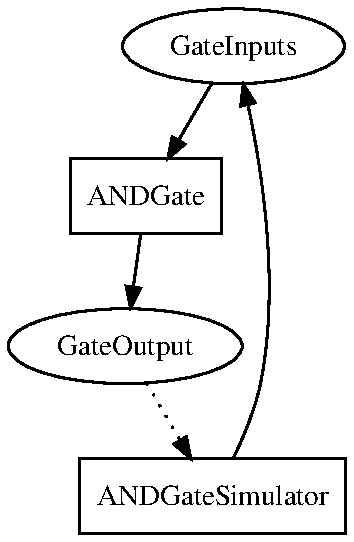
\includegraphics{pictures/ANDGate.pdf}
                \caption{Graphical representation of the AND gate generated by the outputted network.dot file. Here rectangles represent processes and ellipses buses. The arrows show the direction of the data flow, where a dotted line indicates data flow to a clocked process, which means that the process is activated on a rising clock edge.}
                \label{fig:ANDGateDOTFile}
            
        \end{figure} 
    
    \subsection{The Decoder}
        In this section we will start by implementing the 2-bit decoder (see \ref{section:Decoder}) and then look at the n-bit implementation. 
        
        First we set up the logic table, as shown in Table \ref{LogicTable:2BitDecoder}. 
        \begin{table}[h!]
            \centering
            \begin{tabular}{|c|c||c|c|c|c|}
                \hline
                \multicolumn{2}{|c||}{\textbf{Input}}& \multicolumn{4}{c|}{\textbf{Output}}                  \\ \hline
                In1        & In0        & Out3 & Out2 & Out1 & Out0 \\ \hline
                0          & 0          & 0    & 0    & 0    & 1    \\ \hline
                0          & 1          & 0    & 0    & 1    & 0    \\ \hline
                1          & 0          & 0    & 1    & 0    & 0    \\ \hline
                1          & 1          & 1    & 0    & 0    & 0    \\ \hline
            \end{tabular}
            \caption{Logic Table of a 2 input decoder, where the binary representation of the input determines which output gets asserted. For example when In1=1, In0=0 output 1 will get asserted as the binary representation for 2 is 10.}
            \label{LogicTable:2BitDecoder}
        \end{table}
    
        We then derive the logic equation from the table: 
        \begin{equation}
        \label{Eq:2Bitdecoder}
                Out0 = \overline{In1} \cdot \overline{In0}, \quad
                Out1 = \overline{In1} \cdot In0, \quad
                Out2 = In1 \cdot \overline{In0}, \quad
                Out3 = In1 \cdot In0
        \end{equation}
        
        We notice from Eq. \ref{Eq:2Bitdecoder} that we need two NOT gates (one each input), four AND gates and four outputs. Since we only have 1 minterm per output no OR gates are necessary.
        We can then create a circuit diagram of the decoder, as shown in Figure \ref{fig:2BitDecoderSchematic} and use it as our design guide when we implement it in SME.
        \begin{figure}[h!]
            \centering
            \subimport{tikz_stuff/}{2BitDecoderSchematic}
            \caption{Schematic of the 2-bit decoder SME project.}
            \label{fig:2BitDecoderSchematic}
        \end{figure}
        
        Starting with the processes, we see that we need two NOT processes. Hereafter we know that each vertical line goes to an AND gate and since there are four, we create four AND processes. Moving on to the buses we see that there are two input buses, two negated input buses and four output buses. Wiring the buses to the processes correctly we end up with the SME implementation as shown in Figure \ref{fig:2BitDecoderSME}. The code can be found following the link in this footnote\footnote{\url{https://github.com/DanielRamyar/Master_Thesis/tree/master/SME_Implementations/Decoder_2_Bit_new_implementation}}
        \begin{figure}[h!]
            \centering
            \subimport{tikz_stuff/}{2BitDecoderSME}
            \caption{Flowchart of decoder SME project. Here the rectangles represent individual processes. The solid arrow represents a bus and the dashed arrow a bus going to a clocked process. Solid dots show extension of the same bus and any crossing lines are not connected.}
            \label{fig:2BitDecoderSME}
        \end{figure}
        
        \subsubsection{The N bit Decoder}
            The N bit decoder SME implementation is not trivial and the solution here is inspired from Carl Johnson's master thesis \cite{CarlSpeciale}. Since SME needs everything to be known at compile time, we need a way of auto-generating code depending on how many bits we want. This is achieved by using C\scalerel*{\#}{X} templates. We notice that the number of NOT gates needed is always the same as the number of inputs, so for an N bit decoder we need N NOT gates.
            Knowing this we can use a for loop in the code generator to generate N NOT gate processes and since each NOT gate only has one corresponding input, we can add the input and output buses to each NOT gate process in each loop iteration. 
            
            Next we notice that the number of AND gates scales as $2^{N}$. Doing the same as for the NOT gates, we can use a loop to generate each AND gate process. However it is not trivial adding the correct input buses to each AND gate process. The way this was solved was to add a nested loop, with indices \texttt{i} for the outer loop and \texttt{j} for the inner loop. \texttt{i} is responsible for creating the correct number of AND gate processes and \texttt{j} is responsible for the correct number of input buses added to these processes. So for N = 2, we have \texttt{i} $=2^{2}=4$ AND gates and \texttt{j}=2 inputs to these.
            
            Lastly we know that each AND gate should have the correct minterm as input e.g. AND1 in \ref{fig:2BitDecoderSME} has \texttt{In0} and NOT(\texttt{In1}) as input, which produces the correct output.
            To do this, we use the conditional operator with the condition \texttt{((i $\gg$ j \& 1) == 1)}, this will ensure that all AND gate processes gets the correct inputs.
            
            A similar approach was used to generate the bus and simulator files and can be found in this footnote\footnote{\url{https://github.com/DanielRamyar/Master_Thesis/tree/master/SME_Implementations/Decoder_n_Bit}}. To change the number of input bits, simply go into all \texttt{.tt} files and change the \texttt{n} variable at the top of the file to the desired number of bits and run the code generation.   
        
    
    \subsection{The Multiplexer}
        In the section we will implement the 2-bit multiplexer (see \ref{section:Multiplexer}) in SME. First we setup the logic table, as shown in Table \ref{LogicTable:2BitMultiplexer}. 
         \begin{table}[h!]
            \centering
            \begin{tabular}{|c|c|c||c|}
                \hline
                \textbf{A} & \textbf{B} & \textbf{S} & \textbf{C} \\ \hline
                0      &     0      &     0      &     0      \\ \hline
                0      &     1      &     0      &     0      \\ \hline
                1      &     0      &     0      &     1      \\ \hline
                1      &     1      &     0      &     1      \\ \hline
                0      &     0      &     1      &     0      \\ \hline
                0      &     1      &     1      &     1      \\ \hline
                1      &     0      &     1      &     0      \\ \hline
                1      &     1      &     1      &     1      \\ \hline
            \end{tabular}
            \caption{Logic Table of a 2 input multiplexer, where A and B are the input bits, S is the select bit, which chooses whether input A or B should be outputted unchanged and C is the output. }
            \label{LogicTable:2BitMultiplexer}
        \end{table}
        
        Hereafter we derive the logic equation from the table:
        
        \begin{equation}
        C = A \cdot \overline{B} \cdot \overline{S} + A \cdot B \cdot \overline{S} + \overline{A} \cdot B \cdot S + A \cdot B \cdot S
        \end{equation}
        this can be reduced to (see \ref{Section:BooleanEquation})
        \begin{equation}
        \label{Eq:2BitMultiplexer}
        C = A\cdot \bar{S} + B\cdot S.
        \end{equation}
        
        We see from Eq. \ref{Eq:2BitMultiplexer} that we need a single NOT gate, two AND gates and a single OR gate. We can then create a circuit diagram of the decoder, as shown in Figure \ref{fig:2BitMultiplexerSchematic} and use it as our design guide when we implement it in SME.
        \begin{figure}[h!]
            \centering
            \subimport{tikz_stuff/}{2BitMultiplexerSchematic}
            \caption{Schematic of the 2-bit multiplexer SME project.}
            \label{fig:2BitMultiplexerSchematic}
        \end{figure}
    
        Starting with the processes, we notice that we only need one NOT process. Hereafter we know that each vertical line goes to an AND gate and since there are two, we create two AND processes. Lastly we know that each horizontal line in the OR plane corresponds to an OR gate, since we only have one we create one OR process.
        Moving on to the buses we see that there are 3 input buses, where we only use the negated signal from one. Next we have two output buses from the AND gates and a single output bus from the OR gate, that is 7 buses in total we have to create. Wiring the buses to the processes correctly we end up with the SME implementation as shown in Figure \ref{fig:2BitMultiplexerSME}. The code can be found following the link in this footnote \footnote{\url{https://github.com/DanielRamyar/Master_Thesis/tree/master/SME_Implementations/Multiplexer_2_Input}}  
    
        \begin{figure}[h!]
            \centering
            \subimport{tikz_stuff/}{2BitMultiplexerSME}
            \caption{Flowchart of multiplexer SME project. Here the rectangles represent individual processes. The solid arrow represents a bus and the dashed arrow a bus going to a clocked process. Solid dots show extension of the same bus and any crossing lines are not connected.}
            \label{fig:2BitMultiplexerSME}
        \end{figure}
    
    \subsection{Full Adder}
        No general purpose CPU would be any good if it could not add two numbers together. This is why we will go through a gate level implementation of an adder unit in SME. Doing this will also give the reader a good intuition on how the arithmetic logic unit (ALU) works, when we later move away from this approach and let the C\scalerel*{\#}{X} compiler do the work for us and the gate level implementation is "hidden".
        
        As always we start by writing up a logic table with the correct function, which has been done in Table \ref{LogicTable:1BitFullAdder}. The idea is that by chaining multiple 2-bit full adders, we will be able to create an n-bit adder. Therefore each unit contains a carry input and a carry output. The rest is just a matter of asserting the sum output depending on the sum of bits in the inputs. For example in row 3 (not counting the label row) in Table \ref{LogicTable:1BitFullAdder}, we see that only input B is asserted, then it follow from addition $A+B+CarryIn=1$ hence the sum has to be asserted. If the result exceeds 1-bit e.g $1+1=10$ in binary, the CarryOut signal is asserted and sum output deasserted. Following this approach the whole table an be filled.
        
        \begin{table}[h!]
            \centering
            \begin{tabular}{|c|c|c||c|c|}
                \hline
                \textbf{A} & \textbf{B} & \textbf{CarryIn} & \textbf{CarryOut} & \textbf{SUM} \\ \hline
                0      &     0      &        0         &         0         &      0       \\ \hline
                0      &     0      &        1         &         0         &      1       \\ \hline
                0      &     1      &        0         &         0         &      1       \\ \hline
                0      &     1      &        1         &         1         &      0       \\ \hline
                1      &     0      &        0         &         0         &      1       \\ \hline
                1      &     0      &        1         &         1         &      0       \\ \hline
                1      &     1      &        0         &         1         &      0       \\ \hline
                1      &     1      &        1         &         1         &      1       \\ \hline
            \end{tabular}
            \caption{Logic Table of a 2 input multiplexer, where A and B are the input bits, S is the select bit, which chooses whether input A or B should be outputted unchanged and C is the output. }
            \label{LogicTable:1BitFullAdder}
        \end{table}
        
        Now deriving the logic equations from the table we get the following for the CarryOut signal:
        \begin{equation}
            CarryOut = B \cdot CarryIn + A \cdot CarryIn + A \cdot B + A \cdot B \cdot CarryIn
        \end{equation}
        Notice that the negated input has been omitted. This can be done as adding these just results in the last term, so removing these doesn't change the output. Simplifying the expression
        \begin{equation}
            CarryOut = B \cdot CarryIn + A \cdot CarryIn + A \cdot B (1 + CarryIn),
        \end{equation}
        and using that $(1 + CarryIn) = 1$ we get
        \begin{equation}\label{Eq:CarryOut}
            CarryOut = B \cdot CarryIn + A \cdot CarryIn + A \cdot B. 
        \end{equation}
        
        For the SUM signal we get
        \begin{equation}\label{Eq:SUM}
            SUM = \bar{A} \cdot \bar{B} \cdot CarryIn + \bar{A} \cdot B \cdot \overline{CarryIn} + A \cdot \bar{B} \cdot \overline{CarryIn} + A \cdot B \cdot CarryIn.
        \end{equation}
        
        From Eq. \ref{Eq:CarryOut} and \ref{Eq:SUM}, we see that we will need three NOT gates (one for each input), seven AND gates and two OR gates. From this we can then create the circuit diagram for the full adder, which is shown in Figure \ref{fig:1BitFullAdderSchematic}. Hereafter we can use the diagram as our guideline for our SME project.
        
        Starting with the processes, we create 3 NOT gate processes. Hereafter we count seven vertical lines in the AND plane of the schematic, which means we have to make seven AND gate processes. Lastly we see that there are two horizontal lines in OR plane, so we create two OR gate processes.
        
        \begin{figure}[h!]
            \centering
            \subimport{tikz_stuff/}{1BitFullAdder}
            \caption{Schematic of the 2-bit multiplexer SME project.}
            \label{fig:1BitFullAdderSchematic}
        \end{figure}
        
        Moving on to the buses we see that we have 3 input buses and 3 negated input buses. Here we really see the power of SME, since I only have to create a bus once from which all processes can read data from, because of broadcasting (this means i don't have to make a separate copy of the same bus every time a process needs access to it i.e. the bus gets "broadcasted" to all processes). All AND gate processes have an output, so we create 7 output buses for these. Lastly we create the two output buses for the OR gate processes. That is 15 buses in total.  
        
        Wiring the corresponding buses to the correct processes we end up with the SME implementation as shown in Figure \ref{fig:1BitFullAdderSME}. Now this implementation quickly became very complex compared to previous units and this is only for the 2-bit full adder! Realizing that it would be very ambitious project to fully do a gate level implementation of the RISC-V processor, we will move on to another approach discussed in the next section. 
        
        The code can be found following the link in this footnote\footnote{\url{https://github.com/DanielRamyar/Master_Thesis/tree/master/SME_Implementations/FullAdder_2_Bit}}  
    
        \begin{figure}[h!]
            \centering
            \subimport{tikz_stuff/}{1BitFullAdderSME}
            \caption{Flowchart of full adder SME project. Here the rectangles represent individual processes. The solid arrow represents a bus and the dashed arrow a bus going to a clocked process. Solid dots show extension of the same bus and any crossing lines are not connected.}
            \label{fig:1BitFullAdderSME}
        \end{figure}
    
    \subsection{Arithmetic Logic Unit}
        We will in this section move away from the gate level implementation of various units. Instead we will fully utilize the power of C\scalerel*{\#}{X} and let the compiler do most of the work for us. What is meant by this is for example rather than writing a gate level implementation of 64-bit adder, we would instead write a process, which just adds two numbers together using the C\scalerel*{\#}{X} syntax, which simplifies things a whole lot.
        
        The arithmetic logic unit (ALU) is the where all operations happens in the RISC-V architecture. 
        In the following we will go ahead and implement a simple ALU, which can do 4 operations. These operations are addition, subtraction, AND and OR. This will all be contained within the ALU process.
        
        Drawing up a flowchart for the ALU SME project, as we have done in Figure \ref{fig:ALUSME}, we see that the ALU takes 3 input, two lines with data to operate on and one line for selecting the desired operation.
        Now inside the ALU process a \texttt{switch} statement has been made (see Listing \ref{ALUSME}), which uses an operation code coming from the \texttt{OperationCode} bus to determine, which operation it has to do on our data. Hereafter the ALU outputs the result for us to read.
        Now if this had to be implemented using gate level approach, as we did before, it would have quickly been an overwhelming project and is exactly why using a high level language to do the hard work for us is a powerful approach.
        
        The code for this project can be found following the link in this footnote\footnote{\url{https://github.com/DanielRamyar/Master_Thesis/tree/master/SME_Implementations/ALU_1_Bit}}  
        
        
        \begin{figure}[h!]
            \centering
            \subimport{tikz_stuff/}{ALUSME}
            \caption{Flowchart of ALU SME project. Here the rectangles represent individual processes. The solid arrow represents a bus and the dashed arrow a bus going to a clocked process.}
            \label{fig:ALUSME}
        \end{figure}
    
        
        \begin{minipage}{\linewidth}
            \begin{lstlisting}[language={[Sharp]C}, caption={The Ontick() method for the ALU process. Here we use a \texttt{switch} statement, controlled by the \texttt{OperationCode} bus, to determine which operation the ALU should perform. },captionpos=b, label = ALUSME]
protected override void OnTick() {
    switch (m_OperationCode.Value) {
        case 0:
            output.Value = m_A.Value & m_B.Value;
            break;
        case 1:
            output.Value = m_A.Value | m_B.Value;
            break;
        case 2:
            output.Value = m_A.Value + m_B.Value;
            break;
        case 3:
            output.Value = m_A.Value - m_B.Value;
            break;
}
            \end{lstlisting}
      \end{minipage}  
        


    
    
